\section{Structured Observation}
\label{sec:observation}

This section presents the empirical observations from our $5 \times 3$ experimental matrix. We establish three key findings: (1) branch-wise performance structure exists and is significant; (2) logit distillation is suboptimal compared to localization distillation; (3) branch rankings exhibit partial stability across visibility levels, with notable exceptions under heavy degradation.

\subsection{Core Performance Matrix}

\Cref{tab:core_matrix} presents the complete performance matrix across all KD branches and visibility levels. Several patterns are immediately apparent.

\begin{table}[htbp]
\centering
\caption{Core performance matrix (mAP@50) across KD branches and visibility levels. Best result in each column is bolded.}
\label{tab:core_matrix}
\begin{tabular}{@{}lccc@{}}
\toprule
KD Branch & Light ($\beta=0.005$) & Moderate ($\beta=0.01$) & Heavy ($\beta=0.02$) \\
\midrule
student\_only (baseline) & 0.5828 & 0.5873 & 0.5625 \\
logit\_only & 0.5866 & 0.5811 & 0.5678 \\
feature\_only & 0.5861 & 0.5874 & 0.5576 \\
attention\_only & 0.5853 & 0.5776 & \textbf{0.5721} \\
\textbf{localization\_only} & \textbf{0.5952} & \textbf{0.5906} & 0.5606 \\
\bottomrule
\end{tabular}
\end{table}

\textbf{Finding 1: Branch-wise structure exists.} Performance is not uniform across branches. Localization distillation achieves the highest mAP@50 under light and moderate visibility (0.5952 and 0.5906 respectively), while attention distillation performs best under heavy visibility (0.5721). This demonstrates that different KD mechanisms respond distinctly to visibility degradation.

\textbf{Finding 2: Logit distillation is suboptimal.} Despite being the most prevalent KD formulation in the literature, logit distillation achieves only modest performance (0.5866 light, 0.5678 heavy) and never leads the branch comparison. This confirms that conventional output-matching approaches are not optimal for visibility-degraded conditions.

\textbf{Finding 3: Visibility degradation impacts branches differentially.} Under heavy fog ($\beta=0.02$), performance drops are pronounced but uneven: feature distillation drops to 0.5576 (below baseline), while attention distillation improves relative to other branches. This suggests that different knowledge types have varying robustness to visibility loss.

\Cref{fig:branch_performance} visualizes these branch-wise performance patterns.

\begin{figure}[htbp]
\centering
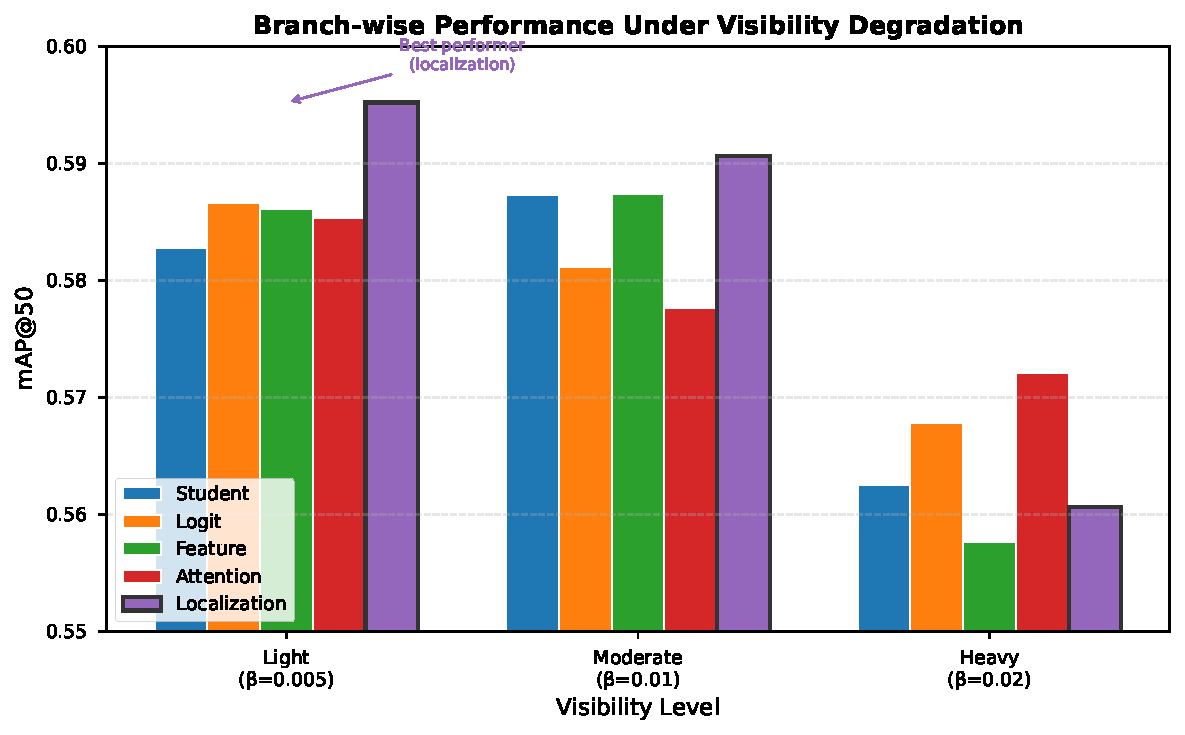
\includegraphics[width=0.85\columnwidth]{figures/fig2_branch_performance.pdf}
\caption{Branch-wise performance under visibility degradation. Localization distillation achieves highest performance under light and moderate visibility, while all branches converge under heavy degradation.}
\label{fig:branch_performance}
\end{figure}

\subsection{KD Gain Analysis}

To quantify the relative effectiveness of each branch, \cref{tab:gain_matrix} presents KD gains computed against the student-only baseline.

\begin{table}[htbp]
\centering
\caption{KD gain matrix (mAP@50 improvement over student-only baseline). Positive values indicate beneficial transfer; negative values indicate negative transfer.}
\label{tab:gain_matrix}
\begin{tabular}{@{}lccc@{}}
\toprule
KD Branch & Light & Moderate & Heavy \\
\midrule
logit\_only & +0.0038 & $-$0.0062 & +0.0053 \\
feature\_only & +0.0033 & +0.0001 & $-$0.0049 \\
attention\_only & +0.0025 & $-$0.0096 & +0.0096 \\
\textbf{localization\_only} & \textbf{+0.0124} & \textbf{+0.0033} & $-$0.0019 \\
\bottomrule
\end{tabular}
\end{table}

\textbf{Finding 4: Localization distillation provides consistent gains under mild-to-moderate degradation.} With gains of +1.24\% (light) and +0.33\% (moderate), localization distillation is the only branch that consistently improves upon the baseline before heavy degradation sets in.

\textbf{Finding 5: Negative transfer occurs.} Feature distillation exhibits negative transfer ($-0.49\%$) under heavy visibility loss, suggesting that direct feature alignment may propagate domain-specific biases that harm student generalization.

\textbf{Finding 6: Heavy degradation eliminates KD benefits.} Under $\beta=0.02$, no branch maintains clear positive gain over the student baseline. This indicates a fundamental limitation: when visibility loss becomes severe, the teacher's knowledge itself degrades, and no distillation mechanism can fully compensate.

\Cref{fig:gain_analysis} visualizes the KD gains relative to the student-only baseline.

\begin{figure}[htbp]
\centering
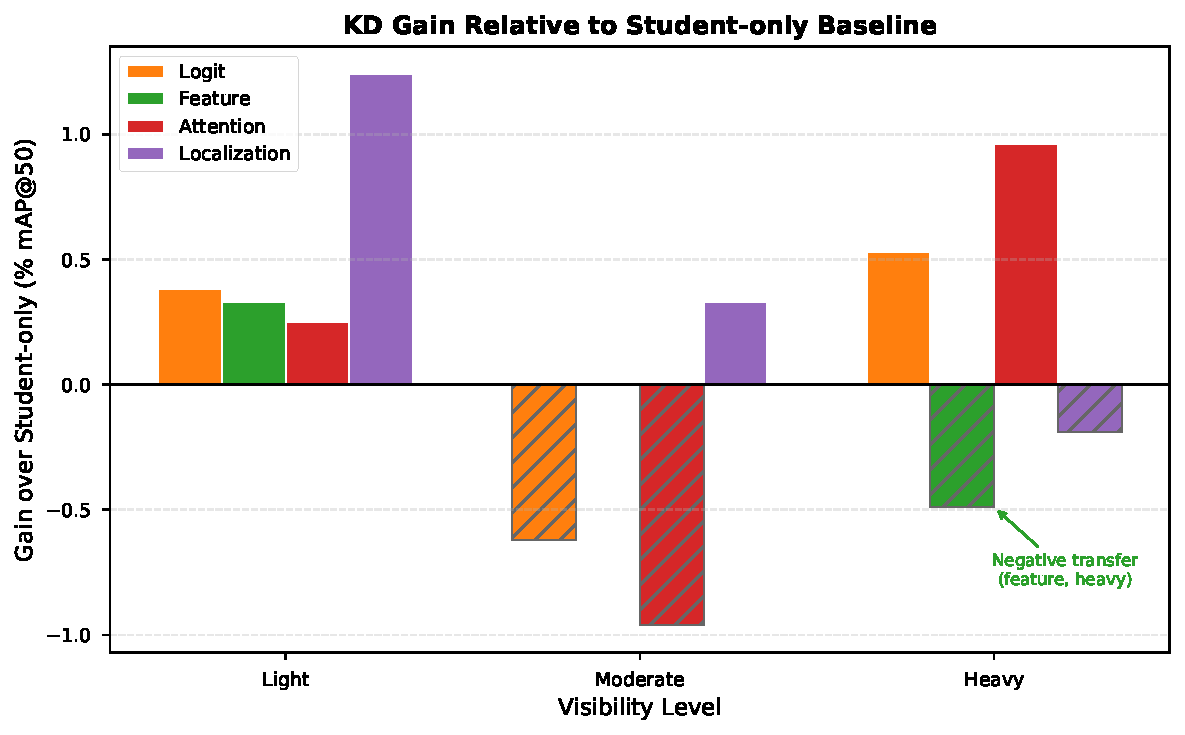
\includegraphics[width=0.85\columnwidth]{figures/fig3_gains.pdf}
\caption{KD gain relative to student-only baseline. Positive values (above dashed line) indicate beneficial transfer; negative values indicate negative transfer. Hatched bars denote negative transfer.}
\label{fig:gain_analysis}
\end{figure}

\subsection{Ranking Stability Analysis}

To assess whether branch-wise structure persists across visibility conditions, we compute Kendall's $\tau$ rank correlation between visibility levels. \Cref{tab:rankings} shows branch rankings at each visibility level.

\begin{table}[htbp]
\centering
\caption{Branch rankings by mAP@50 at each visibility level. Rank 1 is best.}
\label{tab:rankings}
\begin{tabular}{@{}lccccc@{}}
\toprule
Visibility & Rank 1 & Rank 2 & Rank 3 & Rank 4 & Rank 5 \\
\midrule
Light & localization & logit & feature & attention & student \\
Moderate & localization & feature & student & logit & attention \\
Heavy & attention & logit & student & localization & feature \\
\bottomrule
\end{tabular}
\end{table}

Kendall's $\tau$ correlations between rankings:
\begin{itemize}
    \item Light vs. Moderate: $\tau = 0.40$, $p = 0.48$
    \item Moderate vs. Heavy: $\tau = -0.80$, $p = 0.08$
    \item Light vs. Heavy: $\tau = -0.20$, $p = 0.82$
\end{itemize}

\textbf{Finding 7: Partial ranking stability with heavy degradation as an outlier.} The light-to-moderate comparison shows modest positive correlation, suggesting that branch-wise structure partially persists under mild visibility loss. However, heavy degradation produces a fundamentally different ranking ($\tau = -0.80$ vs. moderate), indicating that the mechanisms governing KD effectiveness change qualitatively under severe occlusion.

\subsection{Observation Summary}

Our structured observation phase establishes that:
\begin{enumerate}
    \item Branch-wise performance structure exists and is statistically meaningful;
    \item Logit distillation, despite its prevalence, is not optimal for visibility-degraded detection;
    \item Localization distillation demonstrates relative robustness under mild-to-moderate degradation;
    \item Heavy visibility loss represents a regime change where all KD mechanisms struggle.
\end{enumerate}

These observations motivate the mechanism analysis in \cref{sec:mechanism}, where we test specific hypotheses to explain why these patterns emerge.
